% Created by tikzDevice version 0.12.3.1 on 2022-04-02 11:08:54
% !TEX encoding = UTF-8 Unicode
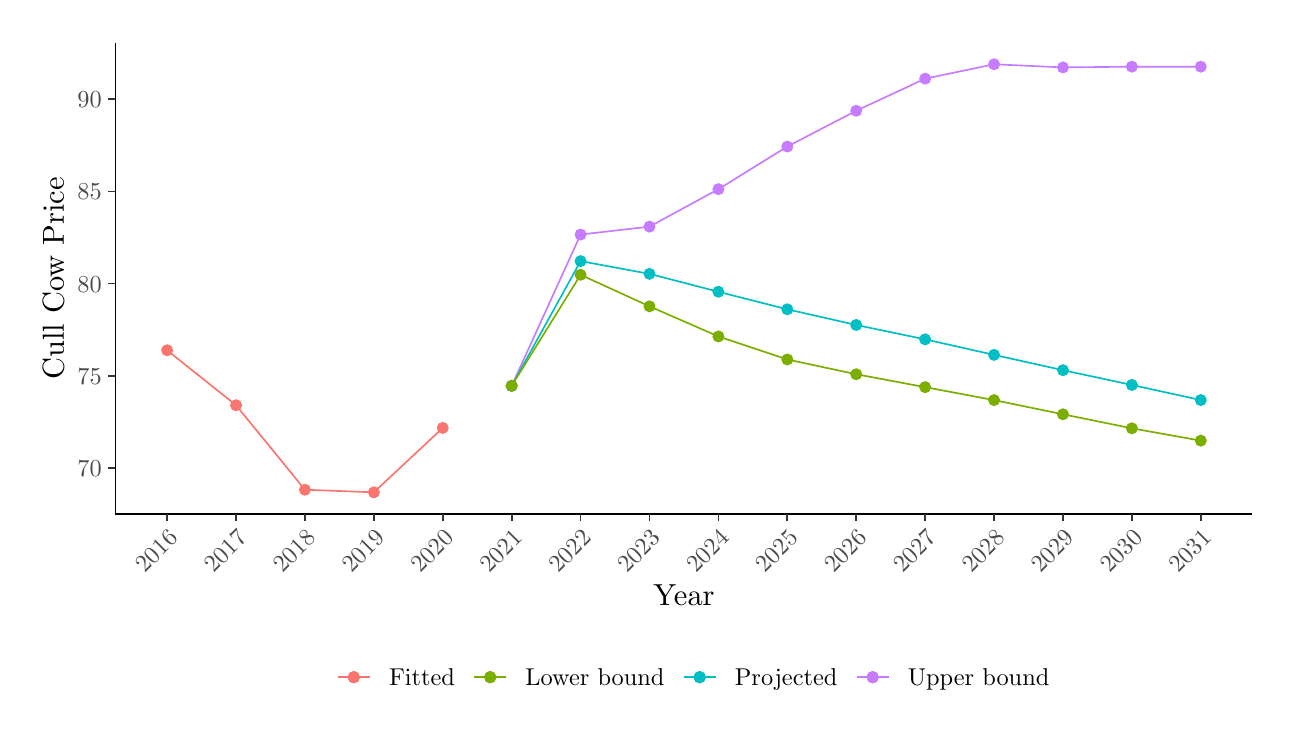
\begin{tikzpicture}[x=1pt,y=1pt]
\definecolor{fillColor}{RGB}{255,255,255}
\path[use as bounding box,fill=fillColor,fill opacity=0.00] (0,0) rectangle (448.07,252.94);
\begin{scope}
\path[clip] (  0.00,  0.00) rectangle (448.07,252.94);
\definecolor{drawColor}{RGB}{255,255,255}
\definecolor{fillColor}{RGB}{255,255,255}

\path[draw=drawColor,line width= 0.6pt,line join=round,line cap=round,fill=fillColor] (  0.00,  0.00) rectangle (448.07,252.94);
\end{scope}
\begin{scope}
\path[clip] ( 31.71, 77.31) rectangle (442.57,247.44);
\definecolor{fillColor}{RGB}{255,255,255}

\path[fill=fillColor] ( 31.71, 77.31) rectangle (442.57,247.44);
\definecolor{drawColor}{RGB}{248,118,109}

\path[draw=drawColor,line width= 0.6pt,line join=round] ( 50.39,136.37) --
	( 75.29,116.51) --
	(100.19, 85.97) --
	(125.09, 85.04) --
	(149.99,108.31);
\definecolor{fillColor}{RGB}{248,118,109}

\path[draw=drawColor,line width= 0.4pt,line join=round,line cap=round,fill=fillColor] ( 50.39,136.37) circle (  1.96);

\path[draw=drawColor,line width= 0.4pt,line join=round,line cap=round,fill=fillColor] ( 75.29,116.51) circle (  1.96);

\path[draw=drawColor,line width= 0.4pt,line join=round,line cap=round,fill=fillColor] (100.19, 85.97) circle (  1.96);

\path[draw=drawColor,line width= 0.4pt,line join=round,line cap=round,fill=fillColor] (125.09, 85.04) circle (  1.96);

\path[draw=drawColor,line width= 0.4pt,line join=round,line cap=round,fill=fillColor] (149.99,108.31) circle (  1.96);
\definecolor{drawColor}{RGB}{199,124,255}

\path[draw=drawColor,line width= 0.6pt,line join=round] (174.89,123.51) --
	(199.79,178.18) --
	(224.69,181.04) --
	(249.59,194.58) --
	(274.49,209.98) --
	(299.39,222.91) --
	(324.30,234.51) --
	(349.20,239.71) --
	(374.10,238.58) --
	(399.00,238.84) --
	(423.90,238.84);
\definecolor{fillColor}{RGB}{199,124,255}

\path[draw=drawColor,line width= 0.4pt,line join=round,line cap=round,fill=fillColor] (174.89,123.51) circle (  1.96);

\path[draw=drawColor,line width= 0.4pt,line join=round,line cap=round,fill=fillColor] (199.79,178.18) circle (  1.96);

\path[draw=drawColor,line width= 0.4pt,line join=round,line cap=round,fill=fillColor] (224.69,181.04) circle (  1.96);

\path[draw=drawColor,line width= 0.4pt,line join=round,line cap=round,fill=fillColor] (249.59,194.58) circle (  1.96);

\path[draw=drawColor,line width= 0.4pt,line join=round,line cap=round,fill=fillColor] (274.49,209.98) circle (  1.96);

\path[draw=drawColor,line width= 0.4pt,line join=round,line cap=round,fill=fillColor] (299.39,222.91) circle (  1.96);

\path[draw=drawColor,line width= 0.4pt,line join=round,line cap=round,fill=fillColor] (324.30,234.51) circle (  1.96);

\path[draw=drawColor,line width= 0.4pt,line join=round,line cap=round,fill=fillColor] (349.20,239.71) circle (  1.96);

\path[draw=drawColor,line width= 0.4pt,line join=round,line cap=round,fill=fillColor] (374.10,238.58) circle (  1.96);

\path[draw=drawColor,line width= 0.4pt,line join=round,line cap=round,fill=fillColor] (399.00,238.84) circle (  1.96);

\path[draw=drawColor,line width= 0.4pt,line join=round,line cap=round,fill=fillColor] (423.90,238.84) circle (  1.96);
\definecolor{drawColor}{RGB}{0,191,196}

\path[draw=drawColor,line width= 0.6pt,line join=round] (174.89,123.51) --
	(199.79,168.58) --
	(224.69,163.98) --
	(249.59,157.51) --
	(274.49,151.17) --
	(299.39,145.51) --
	(324.30,140.31) --
	(349.20,134.71) --
	(374.10,129.17) --
	(399.00,123.84) --
	(423.90,118.37);
\definecolor{fillColor}{RGB}{0,191,196}

\path[draw=drawColor,line width= 0.4pt,line join=round,line cap=round,fill=fillColor] (174.89,123.51) circle (  1.96);

\path[draw=drawColor,line width= 0.4pt,line join=round,line cap=round,fill=fillColor] (199.79,168.58) circle (  1.96);

\path[draw=drawColor,line width= 0.4pt,line join=round,line cap=round,fill=fillColor] (224.69,163.98) circle (  1.96);

\path[draw=drawColor,line width= 0.4pt,line join=round,line cap=round,fill=fillColor] (249.59,157.51) circle (  1.96);

\path[draw=drawColor,line width= 0.4pt,line join=round,line cap=round,fill=fillColor] (274.49,151.17) circle (  1.96);

\path[draw=drawColor,line width= 0.4pt,line join=round,line cap=round,fill=fillColor] (299.39,145.51) circle (  1.96);

\path[draw=drawColor,line width= 0.4pt,line join=round,line cap=round,fill=fillColor] (324.30,140.31) circle (  1.96);

\path[draw=drawColor,line width= 0.4pt,line join=round,line cap=round,fill=fillColor] (349.20,134.71) circle (  1.96);

\path[draw=drawColor,line width= 0.4pt,line join=round,line cap=round,fill=fillColor] (374.10,129.17) circle (  1.96);

\path[draw=drawColor,line width= 0.4pt,line join=round,line cap=round,fill=fillColor] (399.00,123.84) circle (  1.96);

\path[draw=drawColor,line width= 0.4pt,line join=round,line cap=round,fill=fillColor] (423.90,118.37) circle (  1.96);
\definecolor{drawColor}{RGB}{124,174,0}

\path[draw=drawColor,line width= 0.6pt,line join=round] (174.89,123.51) --
	(199.79,163.64) --
	(224.69,152.24) --
	(249.59,141.37) --
	(274.49,133.04) --
	(299.39,127.71) --
	(324.30,123.04) --
	(349.20,118.37) --
	(374.10,113.24) --
	(399.00,108.17) --
	(423.90,103.71);
\definecolor{fillColor}{RGB}{124,174,0}

\path[draw=drawColor,line width= 0.4pt,line join=round,line cap=round,fill=fillColor] (174.89,123.51) circle (  1.96);

\path[draw=drawColor,line width= 0.4pt,line join=round,line cap=round,fill=fillColor] (199.79,163.64) circle (  1.96);

\path[draw=drawColor,line width= 0.4pt,line join=round,line cap=round,fill=fillColor] (224.69,152.24) circle (  1.96);

\path[draw=drawColor,line width= 0.4pt,line join=round,line cap=round,fill=fillColor] (249.59,141.37) circle (  1.96);

\path[draw=drawColor,line width= 0.4pt,line join=round,line cap=round,fill=fillColor] (274.49,133.04) circle (  1.96);

\path[draw=drawColor,line width= 0.4pt,line join=round,line cap=round,fill=fillColor] (299.39,127.71) circle (  1.96);

\path[draw=drawColor,line width= 0.4pt,line join=round,line cap=round,fill=fillColor] (324.30,123.04) circle (  1.96);

\path[draw=drawColor,line width= 0.4pt,line join=round,line cap=round,fill=fillColor] (349.20,118.37) circle (  1.96);

\path[draw=drawColor,line width= 0.4pt,line join=round,line cap=round,fill=fillColor] (374.10,113.24) circle (  1.96);

\path[draw=drawColor,line width= 0.4pt,line join=round,line cap=round,fill=fillColor] (399.00,108.17) circle (  1.96);

\path[draw=drawColor,line width= 0.4pt,line join=round,line cap=round,fill=fillColor] (423.90,103.71) circle (  1.96);
\end{scope}
\begin{scope}
\path[clip] (  0.00,  0.00) rectangle (448.07,252.94);
\definecolor{drawColor}{RGB}{0,0,0}

\path[draw=drawColor,line width= 0.6pt,line join=round] ( 31.71, 77.31) --
	( 31.71,247.44);
\end{scope}
\begin{scope}
\path[clip] (  0.00,  0.00) rectangle (448.07,252.94);
\definecolor{drawColor}{gray}{0.30}

\node[text=drawColor,anchor=base east,inner sep=0pt, outer sep=0pt, scale=  0.88] at ( 26.76, 90.74) {70};

\node[text=drawColor,anchor=base east,inner sep=0pt, outer sep=0pt, scale=  0.88] at ( 26.76,124.08) {75};

\node[text=drawColor,anchor=base east,inner sep=0pt, outer sep=0pt, scale=  0.88] at ( 26.76,157.41) {80};

\node[text=drawColor,anchor=base east,inner sep=0pt, outer sep=0pt, scale=  0.88] at ( 26.76,190.75) {85};

\node[text=drawColor,anchor=base east,inner sep=0pt, outer sep=0pt, scale=  0.88] at ( 26.76,224.08) {90};
\end{scope}
\begin{scope}
\path[clip] (  0.00,  0.00) rectangle (448.07,252.94);
\definecolor{drawColor}{gray}{0.20}

\path[draw=drawColor,line width= 0.6pt,line join=round] ( 28.96, 93.77) --
	( 31.71, 93.77);

\path[draw=drawColor,line width= 0.6pt,line join=round] ( 28.96,127.11) --
	( 31.71,127.11);

\path[draw=drawColor,line width= 0.6pt,line join=round] ( 28.96,160.44) --
	( 31.71,160.44);

\path[draw=drawColor,line width= 0.6pt,line join=round] ( 28.96,193.78) --
	( 31.71,193.78);

\path[draw=drawColor,line width= 0.6pt,line join=round] ( 28.96,227.11) --
	( 31.71,227.11);
\end{scope}
\begin{scope}
\path[clip] (  0.00,  0.00) rectangle (448.07,252.94);
\definecolor{drawColor}{RGB}{0,0,0}

\path[draw=drawColor,line width= 0.6pt,line join=round] ( 31.71, 77.31) --
	(442.57, 77.31);
\end{scope}
\begin{scope}
\path[clip] (  0.00,  0.00) rectangle (448.07,252.94);
\definecolor{drawColor}{gray}{0.20}

\path[draw=drawColor,line width= 0.6pt,line join=round] ( 50.39, 74.56) --
	( 50.39, 77.31);

\path[draw=drawColor,line width= 0.6pt,line join=round] ( 75.29, 74.56) --
	( 75.29, 77.31);

\path[draw=drawColor,line width= 0.6pt,line join=round] (100.19, 74.56) --
	(100.19, 77.31);

\path[draw=drawColor,line width= 0.6pt,line join=round] (125.09, 74.56) --
	(125.09, 77.31);

\path[draw=drawColor,line width= 0.6pt,line join=round] (149.99, 74.56) --
	(149.99, 77.31);

\path[draw=drawColor,line width= 0.6pt,line join=round] (174.89, 74.56) --
	(174.89, 77.31);

\path[draw=drawColor,line width= 0.6pt,line join=round] (199.79, 74.56) --
	(199.79, 77.31);

\path[draw=drawColor,line width= 0.6pt,line join=round] (224.69, 74.56) --
	(224.69, 77.31);

\path[draw=drawColor,line width= 0.6pt,line join=round] (249.59, 74.56) --
	(249.59, 77.31);

\path[draw=drawColor,line width= 0.6pt,line join=round] (274.49, 74.56) --
	(274.49, 77.31);

\path[draw=drawColor,line width= 0.6pt,line join=round] (299.39, 74.56) --
	(299.39, 77.31);

\path[draw=drawColor,line width= 0.6pt,line join=round] (324.30, 74.56) --
	(324.30, 77.31);

\path[draw=drawColor,line width= 0.6pt,line join=round] (349.20, 74.56) --
	(349.20, 77.31);

\path[draw=drawColor,line width= 0.6pt,line join=round] (374.10, 74.56) --
	(374.10, 77.31);

\path[draw=drawColor,line width= 0.6pt,line join=round] (399.00, 74.56) --
	(399.00, 77.31);

\path[draw=drawColor,line width= 0.6pt,line join=round] (423.90, 74.56) --
	(423.90, 77.31);
\end{scope}
\begin{scope}
\path[clip] (  0.00,  0.00) rectangle (448.07,252.94);
\definecolor{drawColor}{gray}{0.30}

\node[text=drawColor,rotate= 45.00,anchor=base east,inner sep=0pt, outer sep=0pt, scale=  0.88] at ( 54.67, 68.07) {2016};

\node[text=drawColor,rotate= 45.00,anchor=base east,inner sep=0pt, outer sep=0pt, scale=  0.88] at ( 79.57, 68.07) {2017};

\node[text=drawColor,rotate= 45.00,anchor=base east,inner sep=0pt, outer sep=0pt, scale=  0.88] at (104.47, 68.07) {2018};

\node[text=drawColor,rotate= 45.00,anchor=base east,inner sep=0pt, outer sep=0pt, scale=  0.88] at (129.38, 68.07) {2019};

\node[text=drawColor,rotate= 45.00,anchor=base east,inner sep=0pt, outer sep=0pt, scale=  0.88] at (154.28, 68.07) {2020};

\node[text=drawColor,rotate= 45.00,anchor=base east,inner sep=0pt, outer sep=0pt, scale=  0.88] at (179.18, 68.07) {2021};

\node[text=drawColor,rotate= 45.00,anchor=base east,inner sep=0pt, outer sep=0pt, scale=  0.88] at (204.08, 68.07) {2022};

\node[text=drawColor,rotate= 45.00,anchor=base east,inner sep=0pt, outer sep=0pt, scale=  0.88] at (228.98, 68.07) {2023};

\node[text=drawColor,rotate= 45.00,anchor=base east,inner sep=0pt, outer sep=0pt, scale=  0.88] at (253.88, 68.07) {2024};

\node[text=drawColor,rotate= 45.00,anchor=base east,inner sep=0pt, outer sep=0pt, scale=  0.88] at (278.78, 68.07) {2025};

\node[text=drawColor,rotate= 45.00,anchor=base east,inner sep=0pt, outer sep=0pt, scale=  0.88] at (303.68, 68.07) {2026};

\node[text=drawColor,rotate= 45.00,anchor=base east,inner sep=0pt, outer sep=0pt, scale=  0.88] at (328.58, 68.07) {2027};

\node[text=drawColor,rotate= 45.00,anchor=base east,inner sep=0pt, outer sep=0pt, scale=  0.88] at (353.48, 68.07) {2028};

\node[text=drawColor,rotate= 45.00,anchor=base east,inner sep=0pt, outer sep=0pt, scale=  0.88] at (378.38, 68.07) {2029};

\node[text=drawColor,rotate= 45.00,anchor=base east,inner sep=0pt, outer sep=0pt, scale=  0.88] at (403.28, 68.07) {2030};

\node[text=drawColor,rotate= 45.00,anchor=base east,inner sep=0pt, outer sep=0pt, scale=  0.88] at (428.18, 68.07) {2031};
\end{scope}
\begin{scope}
\path[clip] (  0.00,  0.00) rectangle (448.07,252.94);
\definecolor{drawColor}{RGB}{0,0,0}

\node[text=drawColor,anchor=base,inner sep=0pt, outer sep=0pt, scale=  1.10] at (237.14, 44.09) {Year};
\end{scope}
\begin{scope}
\path[clip] (  0.00,  0.00) rectangle (448.07,252.94);
\definecolor{drawColor}{RGB}{0,0,0}

\node[text=drawColor,rotate= 90.00,anchor=base,inner sep=0pt, outer sep=0pt, scale=  1.10] at ( 13.08,162.38) {Cull Cow Price};
\end{scope}
\begin{scope}
\path[clip] (  0.00,  0.00) rectangle (448.07,252.94);
\definecolor{fillColor}{RGB}{255,255,255}

\path[fill=fillColor] ( 99.62,  5.50) rectangle (374.66, 30.95);
\end{scope}
\begin{scope}
\path[clip] (  0.00,  0.00) rectangle (448.07,252.94);
\definecolor{drawColor}{RGB}{248,118,109}

\path[draw=drawColor,line width= 0.6pt,line join=round] (112.07, 18.23) -- (123.63, 18.23);
\end{scope}
\begin{scope}
\path[clip] (  0.00,  0.00) rectangle (448.07,252.94);
\definecolor{drawColor}{RGB}{248,118,109}
\definecolor{fillColor}{RGB}{248,118,109}

\path[draw=drawColor,line width= 0.4pt,line join=round,line cap=round,fill=fillColor] (117.85, 18.23) circle (  1.96);
\end{scope}
\begin{scope}
\path[clip] (  0.00,  0.00) rectangle (448.07,252.94);
\definecolor{drawColor}{RGB}{248,118,109}

\path[draw=drawColor,line width= 0.6pt,line join=round] (112.07, 18.23) -- (123.63, 18.23);
\end{scope}
\begin{scope}
\path[clip] (  0.00,  0.00) rectangle (448.07,252.94);
\definecolor{drawColor}{RGB}{248,118,109}
\definecolor{fillColor}{RGB}{248,118,109}

\path[draw=drawColor,line width= 0.4pt,line join=round,line cap=round,fill=fillColor] (117.85, 18.23) circle (  1.96);
\end{scope}
\begin{scope}
\path[clip] (  0.00,  0.00) rectangle (448.07,252.94);
\definecolor{drawColor}{RGB}{248,118,109}

\path[draw=drawColor,line width= 0.6pt,line join=round] (112.07, 18.23) -- (123.63, 18.23);
\end{scope}
\begin{scope}
\path[clip] (  0.00,  0.00) rectangle (448.07,252.94);
\definecolor{drawColor}{RGB}{248,118,109}
\definecolor{fillColor}{RGB}{248,118,109}

\path[draw=drawColor,line width= 0.4pt,line join=round,line cap=round,fill=fillColor] (117.85, 18.23) circle (  1.96);
\end{scope}
\begin{scope}
\path[clip] (  0.00,  0.00) rectangle (448.07,252.94);
\definecolor{drawColor}{RGB}{248,118,109}

\path[draw=drawColor,line width= 0.6pt,line join=round] (112.07, 18.23) -- (123.63, 18.23);
\end{scope}
\begin{scope}
\path[clip] (  0.00,  0.00) rectangle (448.07,252.94);
\definecolor{drawColor}{RGB}{248,118,109}
\definecolor{fillColor}{RGB}{248,118,109}

\path[draw=drawColor,line width= 0.4pt,line join=round,line cap=round,fill=fillColor] (117.85, 18.23) circle (  1.96);
\end{scope}
\begin{scope}
\path[clip] (  0.00,  0.00) rectangle (448.07,252.94);
\definecolor{drawColor}{RGB}{124,174,0}

\path[draw=drawColor,line width= 0.6pt,line join=round] (161.35, 18.23) -- (172.91, 18.23);
\end{scope}
\begin{scope}
\path[clip] (  0.00,  0.00) rectangle (448.07,252.94);
\definecolor{drawColor}{RGB}{124,174,0}
\definecolor{fillColor}{RGB}{124,174,0}

\path[draw=drawColor,line width= 0.4pt,line join=round,line cap=round,fill=fillColor] (167.13, 18.23) circle (  1.96);
\end{scope}
\begin{scope}
\path[clip] (  0.00,  0.00) rectangle (448.07,252.94);
\definecolor{drawColor}{RGB}{124,174,0}

\path[draw=drawColor,line width= 0.6pt,line join=round] (161.35, 18.23) -- (172.91, 18.23);
\end{scope}
\begin{scope}
\path[clip] (  0.00,  0.00) rectangle (448.07,252.94);
\definecolor{drawColor}{RGB}{124,174,0}
\definecolor{fillColor}{RGB}{124,174,0}

\path[draw=drawColor,line width= 0.4pt,line join=round,line cap=round,fill=fillColor] (167.13, 18.23) circle (  1.96);
\end{scope}
\begin{scope}
\path[clip] (  0.00,  0.00) rectangle (448.07,252.94);
\definecolor{drawColor}{RGB}{124,174,0}

\path[draw=drawColor,line width= 0.6pt,line join=round] (161.35, 18.23) -- (172.91, 18.23);
\end{scope}
\begin{scope}
\path[clip] (  0.00,  0.00) rectangle (448.07,252.94);
\definecolor{drawColor}{RGB}{124,174,0}
\definecolor{fillColor}{RGB}{124,174,0}

\path[draw=drawColor,line width= 0.4pt,line join=round,line cap=round,fill=fillColor] (167.13, 18.23) circle (  1.96);
\end{scope}
\begin{scope}
\path[clip] (  0.00,  0.00) rectangle (448.07,252.94);
\definecolor{drawColor}{RGB}{124,174,0}

\path[draw=drawColor,line width= 0.6pt,line join=round] (161.35, 18.23) -- (172.91, 18.23);
\end{scope}
\begin{scope}
\path[clip] (  0.00,  0.00) rectangle (448.07,252.94);
\definecolor{drawColor}{RGB}{124,174,0}
\definecolor{fillColor}{RGB}{124,174,0}

\path[draw=drawColor,line width= 0.4pt,line join=round,line cap=round,fill=fillColor] (167.13, 18.23) circle (  1.96);
\end{scope}
\begin{scope}
\path[clip] (  0.00,  0.00) rectangle (448.07,252.94);
\definecolor{drawColor}{RGB}{0,191,196}

\path[draw=drawColor,line width= 0.6pt,line join=round] (237.05, 18.23) -- (248.61, 18.23);
\end{scope}
\begin{scope}
\path[clip] (  0.00,  0.00) rectangle (448.07,252.94);
\definecolor{drawColor}{RGB}{0,191,196}
\definecolor{fillColor}{RGB}{0,191,196}

\path[draw=drawColor,line width= 0.4pt,line join=round,line cap=round,fill=fillColor] (242.83, 18.23) circle (  1.96);
\end{scope}
\begin{scope}
\path[clip] (  0.00,  0.00) rectangle (448.07,252.94);
\definecolor{drawColor}{RGB}{0,191,196}

\path[draw=drawColor,line width= 0.6pt,line join=round] (237.05, 18.23) -- (248.61, 18.23);
\end{scope}
\begin{scope}
\path[clip] (  0.00,  0.00) rectangle (448.07,252.94);
\definecolor{drawColor}{RGB}{0,191,196}
\definecolor{fillColor}{RGB}{0,191,196}

\path[draw=drawColor,line width= 0.4pt,line join=round,line cap=round,fill=fillColor] (242.83, 18.23) circle (  1.96);
\end{scope}
\begin{scope}
\path[clip] (  0.00,  0.00) rectangle (448.07,252.94);
\definecolor{drawColor}{RGB}{0,191,196}

\path[draw=drawColor,line width= 0.6pt,line join=round] (237.05, 18.23) -- (248.61, 18.23);
\end{scope}
\begin{scope}
\path[clip] (  0.00,  0.00) rectangle (448.07,252.94);
\definecolor{drawColor}{RGB}{0,191,196}
\definecolor{fillColor}{RGB}{0,191,196}

\path[draw=drawColor,line width= 0.4pt,line join=round,line cap=round,fill=fillColor] (242.83, 18.23) circle (  1.96);
\end{scope}
\begin{scope}
\path[clip] (  0.00,  0.00) rectangle (448.07,252.94);
\definecolor{drawColor}{RGB}{0,191,196}

\path[draw=drawColor,line width= 0.6pt,line join=round] (237.05, 18.23) -- (248.61, 18.23);
\end{scope}
\begin{scope}
\path[clip] (  0.00,  0.00) rectangle (448.07,252.94);
\definecolor{drawColor}{RGB}{0,191,196}
\definecolor{fillColor}{RGB}{0,191,196}

\path[draw=drawColor,line width= 0.4pt,line join=round,line cap=round,fill=fillColor] (242.83, 18.23) circle (  1.96);
\end{scope}
\begin{scope}
\path[clip] (  0.00,  0.00) rectangle (448.07,252.94);
\definecolor{drawColor}{RGB}{199,124,255}

\path[draw=drawColor,line width= 0.6pt,line join=round] (299.55, 18.23) -- (311.12, 18.23);
\end{scope}
\begin{scope}
\path[clip] (  0.00,  0.00) rectangle (448.07,252.94);
\definecolor{drawColor}{RGB}{199,124,255}
\definecolor{fillColor}{RGB}{199,124,255}

\path[draw=drawColor,line width= 0.4pt,line join=round,line cap=round,fill=fillColor] (305.33, 18.23) circle (  1.96);
\end{scope}
\begin{scope}
\path[clip] (  0.00,  0.00) rectangle (448.07,252.94);
\definecolor{drawColor}{RGB}{199,124,255}

\path[draw=drawColor,line width= 0.6pt,line join=round] (299.55, 18.23) -- (311.12, 18.23);
\end{scope}
\begin{scope}
\path[clip] (  0.00,  0.00) rectangle (448.07,252.94);
\definecolor{drawColor}{RGB}{199,124,255}
\definecolor{fillColor}{RGB}{199,124,255}

\path[draw=drawColor,line width= 0.4pt,line join=round,line cap=round,fill=fillColor] (305.33, 18.23) circle (  1.96);
\end{scope}
\begin{scope}
\path[clip] (  0.00,  0.00) rectangle (448.07,252.94);
\definecolor{drawColor}{RGB}{199,124,255}

\path[draw=drawColor,line width= 0.6pt,line join=round] (299.55, 18.23) -- (311.12, 18.23);
\end{scope}
\begin{scope}
\path[clip] (  0.00,  0.00) rectangle (448.07,252.94);
\definecolor{drawColor}{RGB}{199,124,255}
\definecolor{fillColor}{RGB}{199,124,255}

\path[draw=drawColor,line width= 0.4pt,line join=round,line cap=round,fill=fillColor] (305.33, 18.23) circle (  1.96);
\end{scope}
\begin{scope}
\path[clip] (  0.00,  0.00) rectangle (448.07,252.94);
\definecolor{drawColor}{RGB}{199,124,255}

\path[draw=drawColor,line width= 0.6pt,line join=round] (299.55, 18.23) -- (311.12, 18.23);
\end{scope}
\begin{scope}
\path[clip] (  0.00,  0.00) rectangle (448.07,252.94);
\definecolor{drawColor}{RGB}{199,124,255}
\definecolor{fillColor}{RGB}{199,124,255}

\path[draw=drawColor,line width= 0.4pt,line join=round,line cap=round,fill=fillColor] (305.33, 18.23) circle (  1.96);
\end{scope}
\begin{scope}
\path[clip] (  0.00,  0.00) rectangle (448.07,252.94);
\definecolor{drawColor}{RGB}{0,0,0}

\node[text=drawColor,anchor=base west,inner sep=0pt, outer sep=0pt, scale=  0.88] at (130.58, 15.20) {Fitted};
\end{scope}
\begin{scope}
\path[clip] (  0.00,  0.00) rectangle (448.07,252.94);
\definecolor{drawColor}{RGB}{0,0,0}

\node[text=drawColor,anchor=base west,inner sep=0pt, outer sep=0pt, scale=  0.88] at (179.86, 15.20) {Lower bound};
\end{scope}
\begin{scope}
\path[clip] (  0.00,  0.00) rectangle (448.07,252.94);
\definecolor{drawColor}{RGB}{0,0,0}

\node[text=drawColor,anchor=base west,inner sep=0pt, outer sep=0pt, scale=  0.88] at (255.56, 15.20) {Projected};
\end{scope}
\begin{scope}
\path[clip] (  0.00,  0.00) rectangle (448.07,252.94);
\definecolor{drawColor}{RGB}{0,0,0}

\node[text=drawColor,anchor=base west,inner sep=0pt, outer sep=0pt, scale=  0.88] at (318.06, 15.20) {Upper bound};
\end{scope}
\end{tikzpicture}
